\section{Experimental Results}
\label{sec:results}

\begin{figure}
  \centering
  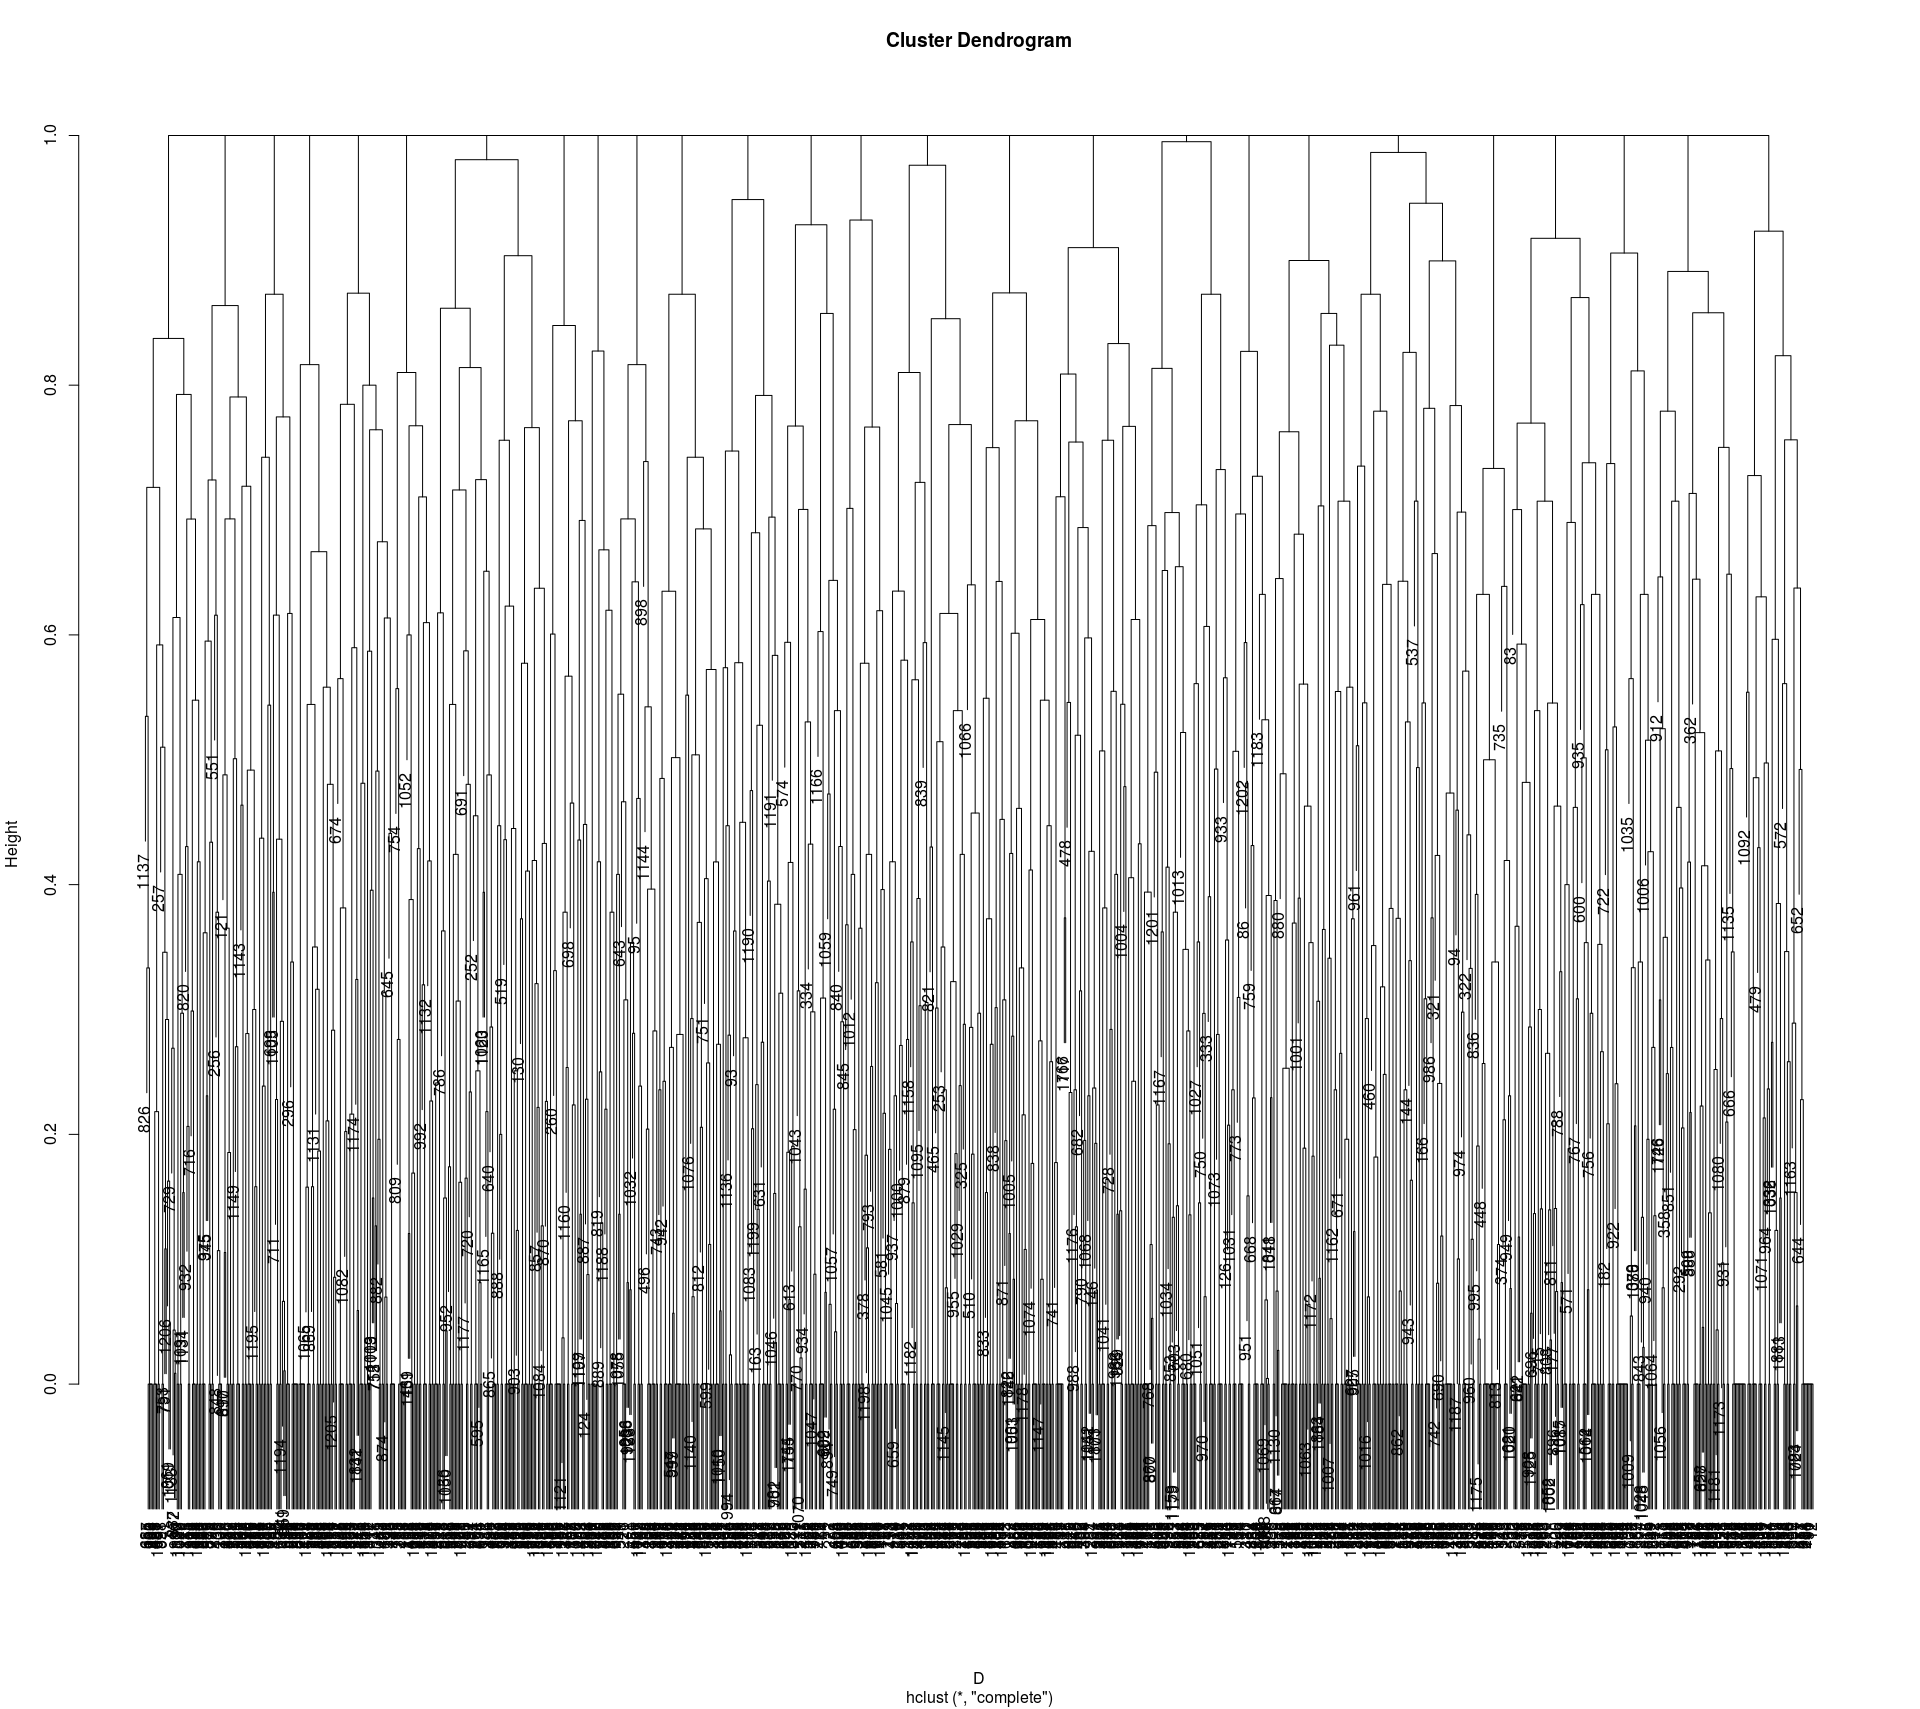
\includegraphics[width=0.5\textwidth]{pictures/clust.png}
  \caption{The dendrogram produced by hierarchical clustering}
  \label{fig:clust}
\end{figure}

Due to the restrictions imposed by the GitHub APIs, we were able to generate only a fairly small dataset. We ran our system three times, until we finished the available API calls, to collect a final dataset of 2762 samples from 107 different repositories. We applied hierarchical clustering on this dataset. The resulting dendrogram is shown in Figure \ref{fig:clust}. We can see that the cluster distribution is not completely random but we are able to distiguish some clusters. In particular, a cutting point of 30 clusters seems to be the best according to the dendrogram. We decided to evaluate our clusters by using the repository ID from which each sample is generated. In particular, we augmented each sample with its repository ID and, given the 30 clusters produced by hierarchical clustering, we computed the entropy based on such variable. We obtained an entropy of 0.7. Remembering that 0.5 implies a completely random distribution, 0.7 means that we are able to detect a slight pattern: the repository IDs are not randomly distributed in the clusters, that is, there is some relation between the changes and the project. This may be a sign that developers of the same project tend to repeat the same semantic errors or to apply the same semantic corrections. Notice however that we would need much more samples to confirm this argument. At the moment, this was the only technique we could come up with to evaluate our clusters, since our initial idea to use bug reports was not feasible. 
